%!Tex Root = ../Tutorat4.tex
% ./Packete.tex
% ./Design.tex
% ./Deklarationen.tex
% ./Aufgabe2.tex
% ./Aufgabe3.tex
% ./Bonus.tex

\section{Task 1}

\setcounter{task}{1}

\begin{frame}[allowframebreaks]{Task 1}{Earliest Deadline First (EDF) and Total Bandwidth Server (TBS)}
  \begin{tasknoinc}
    \begin{itemize}
      \item what can be the maximum value of $U_s$ such that the whole set (i.e. periodic tasks and the \alert{TBS}) is schedulable with \alert{EDF}?
    \end{itemize}
  \end{tasknoinc}
  \begin{requirementsnoinc}
    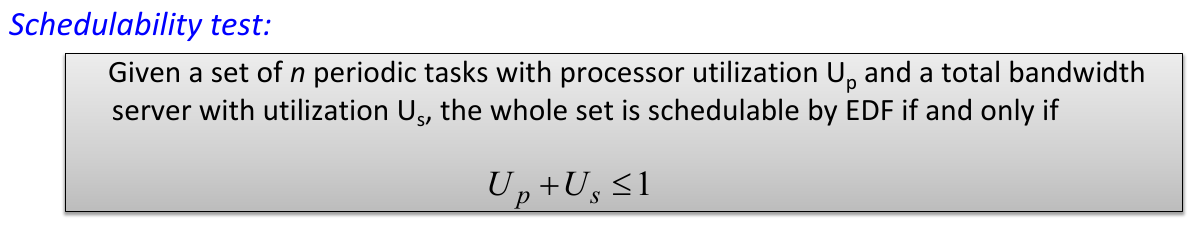
\includegraphics[width=\textwidth]{./figures/schedulability_test.png}
    \begin{itemize}
      \item \alert{processor utilization factor:} $U=\sum_{i=1}^n \frac{C_i}{T_i}$
    \end{itemize}
  \end{requirementsnoinc}
  \begin{solution}
    \begin{itemize}
      \item \alert{Maximum utilization of the Total Bandwidth Server:} $U_{s, \max }=1-U_p=1-(\frac{1}{3}+\frac{1}{5}+\frac{2}{13})=\frac{61}{195} \approx 0.3128$
    \end{itemize}
  \end{solution}
\end{frame}

\begin{frame}[allowframebreaks]{}{}
  \begin{solution}
    \begin{itemize}
      \item First, we need to order the tasks by increasing release time $r_i: J_4, J_6, J_5$. Then, we calculate the deadlines with $d_i=\max \left(r_i, d_{k-1}\right)+\frac{C_k}{U_s}$, where $d_{k-1}$ denotes the previously calculated deadline $(k-1$ means the predecessor in the ordering according to the release time):
  \begin{itemize}
    \item $d_4=\max \left(r_4, d_0\right)+2 / 0.25=0+8=8$
    \item $d_6=\max \left(r_6, d_4\right)+1 / 0.25=10+4=14$
    \item $d_5=\max \left(r_5, d_6\right)+1 / 0.25=15+4=19$
  \end{itemize}
    \end{itemize}
  \end{solution}
  \begin{solution}
    \centering
    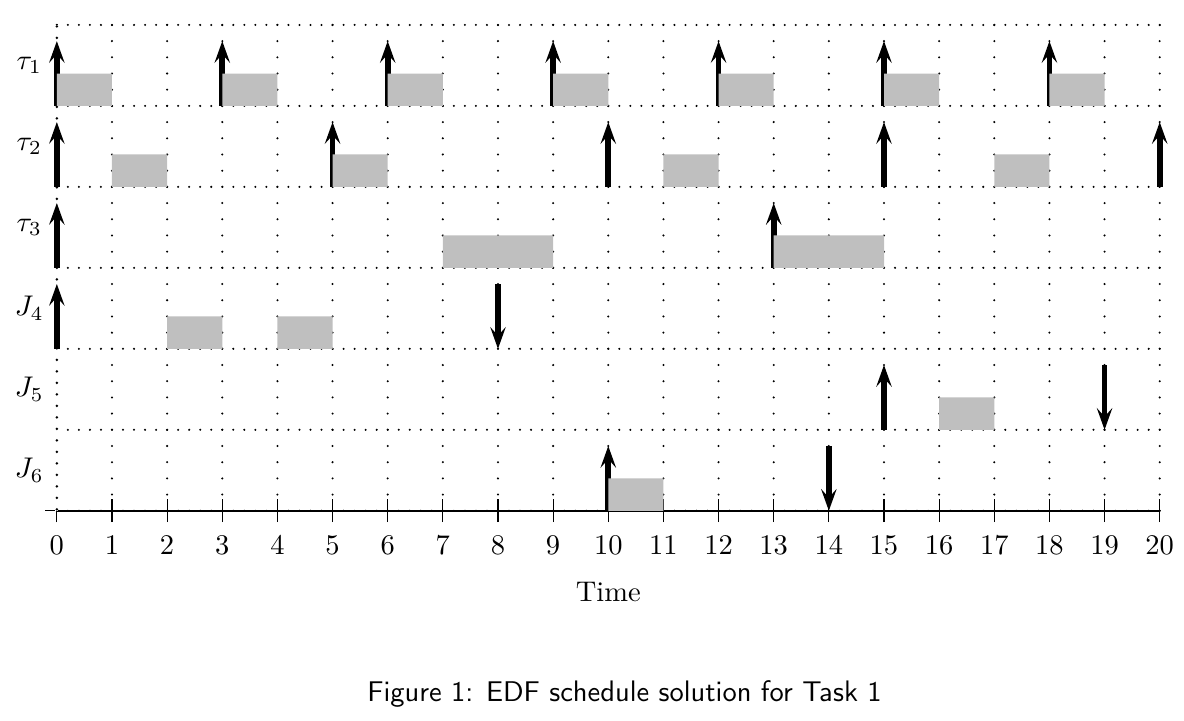
\includegraphics[height=0.6\paperheight]{./figures/1_sol.png}
  \end{solution}
\end{frame}

% \begin{frame}{Mixed Task Sets}{}
%     \begin{itemize}
%         \item So far: we differentiated between \alert{periodic} and \alert{aperiodic} tasks.
%         \item Now: Consider a \alert{mixed} task set!
%         \item We want to be able to find a schedule when there's both \alert{periodic} and \alert{aperiodic} tasks.
%     \end{itemize}
% \end{frame}
%
% \begin{frame}{Schedulability tests}{Sufficient? Necesarry?}
%     \begin{itemize}
%         \item We're interested in whether a given problem can be scheduled by algorithms.
%         \item Depending on the algorithm we can derive sufficient and necesarry conditions.
%         \item[]\alert{Sufficient:} If $A \implies B$ then A is a sufficient condition for B.
%         \item[]\alert{Necesarry:} If $B \implies A$ then A is a necesarry condition for B.
%         \item A necesarry and sufficient condition means, both statements are logically equivalent.
%     \end{itemize}
% \end{frame}
% \begin{frame}{Schedulability tests}{Utilization}
%     Different kind of utilizations also play a big role in our analysis. We introduced the \alert{processor utilization factor} $U = \sum\limits_{i=1}^{n}\cfrac{C_i}{T_i}$ and later on $U_s$ as the server utilization.
%
%     (More about servers later)
% \end{frame}
% \begin{frame}{RM - Rate Monotonic Scheduling}{Schedulability}
% \begin{itemize}
%     \item RM is optimal among all fixed-priority assignments in the sense that no other fixed-priority algorithm can schedule a task set that cannot be scheduled by RM.
%     \item As in the lecture, we have $\sum\limits_{i=1}^{n}\cfrac{C_i}{T_i} \leq n(2^{1/n}-1)$ as a \alert{sufficient} but not \alert{necesarry} condition.
% \end{itemize}
% \end{frame}
% \begin{frame}{RM(PS) - Rate Monotonic Polling Server}
%     \begin{itemize}
%         \item One way to handle both periodic and aperiodic tasks is to use a so called server.
%         \item This PS (Polling Server) acts as a periodic task (meaning it is instantiated at regular intervals $T_s$) whose job it is to, once it has the highest priority, serve any pending aperiodic requests within the limits of a server capacity $C_s$.
%         \item Since we introduce yet another periodic task, the schedulability analysis simply is the same as normal $RM$ with one additional task. Again, we have the \alert{sufficient} but not \alert{necesarry} condition: $\cfrac{C_s}{T_s} + \sum\limits_{i=1}^{n}\cfrac{C_i}{T_i} \leq (n+1)(2^{1/(n+1)}-1)$
%     \end{itemize}
% \end{frame}
%
% \begin{frame}{EDF - Total Bandwidth Server}
%
% \end{frame}
